\documentclass[a0paper,portrait]{baposter}

\usepackage{xcolor}
\usepackage{wrapfig}
\usepackage{lmodern}
\usepackage{lipsum,graphicx}
\usepackage[utf8]{inputenc} %unicode support
\usepackage[T1]{fontenc}

\selectcolormodel{cmyk}

\graphicspath{{figures/}} % Directory in which figures are stored

\newcommand{\compresslist}{%
\setlength{\itemsep}{0pt}%
\setlength{\parskip}{1pt}%
\setlength{\parsep}{0pt}%
}

\newenvironment{boenumerate}
  {\begin{enumerate}\renewcommand\labelenumi{\textbf\theenumi.}}
  {\end{enumerate}}


\begin{document}

\definecolor{Mycolor1}{HTML}{B19D60} 

\definecolor{Mycolor2}{HTML}{FFDF00} 

\definecolor{Mycolor3}{HTML}{234DEB} 

\begin{poster}
{
grid=false,
headerborder=open, % Adds a border around the header of content boxes
colspacing=1em, % Column spacing
bgColorOne=white, % Background color for the gradient on the left side of the poster
bgColorTwo=white, % Background color for the gradient on the right side of the poster
borderColor=Mycolor1, % Border color
headerColorOne=Mycolor2, % Background color for the header in the content boxes (left side)
headerColorTwo=Mycolor2, % Background color for the header in the content boxes (right side)
headerFontColor=Mycolor3, % Text color for the header text in the content boxes
boxColorOne=white, % Background color of the content boxes
textborder=rounded, %rectangle, % Format of the border around content boxes, can be: none, bars, coils, triangles, rectangle, rounded, roundedsmall, roundedright or faded
eyecatcher=false, % Set to false for ignoring the left logo in the title and move the title left
headerheight=0.11\textheight, % Height of the header
headershape=rounded, % Specify the rounded corner in the content box headers, can be: rectangle, small-rounded, roundedright, roundedleft or rounded
headershade=plain,
headerfont=\Large\textsf, % Large, bold and sans serif font in the headers of content boxes
%textfont={\setlength{\parindent}{1.5em}}, % Uncomment for paragraph indentation
linewidth=2pt % Width of the border lines around content boxes
}
{}
%
%----------------------------------------------------------------------------------------
%	TITLE AND AUTHOR NAME
%----------------------------------------------------------------------------------------
%
{
  \textsf %Sans Serif
  {
    \hspace{-0.7cm}
    {CanAir.io}
  }
} % Poster title
% {\vspace{0.2em} Add Author Name, Add another author name\\ 
% {\small \vspace{0.7em} Department of Computing, TU Dublin, Tallaght, Dublin, Ireland}} 
{\sf\vspace{0.2em}\\
Antonio Vanegas  % Author names
\vspace{0.1em}\\
\small{ CanAirIO founder, Android-Hardware developer, Cos4Cloud member
\vspace{0.2em}\\
@hpsaturn  % Author email addresses
}
}
{
\includegraphics[width=.14\linewidth]{images/logo.png}} % CanAir.io logo


% this states the box starts at column 0 (edge of page), row 0 (top of page) for a span of 3 (columns wide)
\headerbox{CanAirIO Citizen Network for Air Quality Monitoring}{name=introduction,column=0,row=0, span=3}{
  Open Source initiative that uses a ESP32 module and different
  PM2.5 sensors, interfaced with an Android client app to have static (WiFi) or mobile
  (Bluetooth) air quality stations. 
\vspace{0.5em}\\
  CanAirIO is a citizen science iniciative that not only aims to generate an air
  quality network of fixed monitoring stations, but also to measure what occurs
  with pedestrians, drivers and passengers in their daily lives considering that
  in some cities with high population density the most affected people are moving. 
  For this reason, we are developing a mobile application that is able to set a PM2.5
  sensor, and other related sensors from the smartphone as fixed station or mobile
  reporter.

%\vspace{2cm} %remove this, only added for spacing

}

% this states the box starts at column 0 (edge of page), directly below the box labelled introduction for a span of 1 (column wide)
\headerbox{Main Goals}{name=subtopic1,column=0,below=introduction,span=1}{

  - To conform a global air quality network
  \vspace{0.1em}\\
  - Mobile visualizations on real time
  \vspace{0.1em}\\
  - Unification and joining with other iniciatives
  \vspace{0.1em}\\
  - Cripto currency incentives to reporters
  \vspace{0.1em}\\
  - To improve device creation usability
  \vspace{0.1em}\\
  - To find partners for hardware co-creations
  \vspace{0.1em}\\
  
  
  \vspace{1.8cm}

}

% this states the box starts at column 0 (edge of page), directly below the box labelled subtopic1 for a span of 1 (column wide)

\headerbox{CanAirIO in the World}{name=subtopic2,column=0,below=subtopic1,span=1}{

  \vspace{0.1cm}
  
  We want improve the DIY hardware and reduce the sensor complexity to
  help more people in the world.

  \vspace{0.1cm}

  {
    \hspace{-0.1cm}
    \centering
    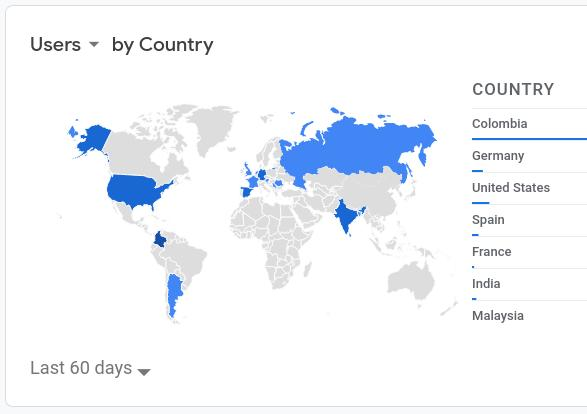
\includegraphics[scale=.28]{images/user_countries20200309.jpg}
  }
}

\headerbox{OpenSource and OpenHardware project}{name=subtopic3,column=1,below=introduction,span=2}{
  \vspace{0.1cm}

  % inserts an image inside the box, 5 rows high
  \begin{wrapfigure}[4]{r}{0.5\textwidth}
    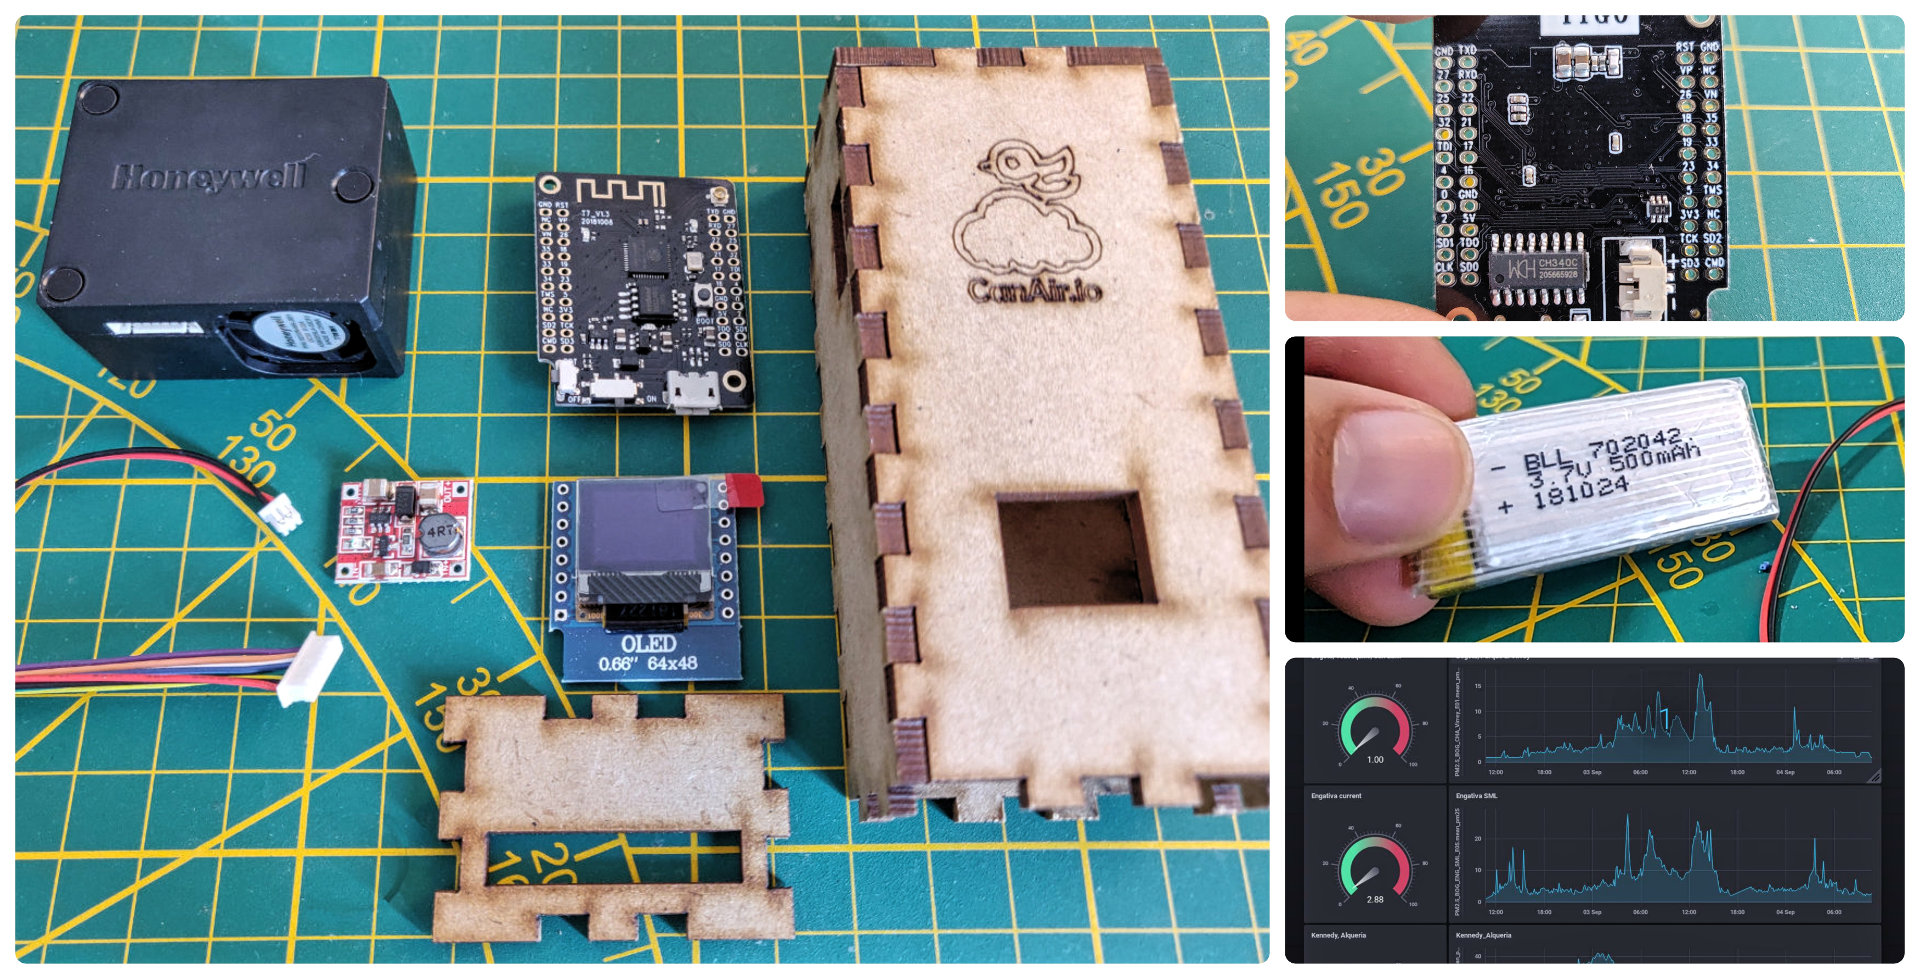
\includegraphics[width=1\linewidth]{images/canariov2collage01.jpg} 
  \end{wrapfigure}

  \subsubsection*{Development status:} 

  - Multiple sensor devices are supported.
  \vspace{0.1em}\\
  - WiFi and sensor setup via BLE.
  \vspace{0.1em}\\
  - All firmware in PlatformIO framework.
  \vspace{0.1em}\\
  - Android native application (GATT client)
  \vspace{0.1em}\\
  - 3DPrint and Laser cut case for mobile.

  \subsubsection*{Community status:} 
  
  - Aprox 100 sensors (maybe more).
  \vspace{0.1em}\\
  - Open InfluxDB cloud server.
  \vspace{0.1em}\\
  - API for writing; reading in development.
  \vspace{0.1em}\\
  - Real time map and static data visualizations.
  \vspace{0.1em}\\
  - Tool to show dynamic tracks for mobile captures. 
  \vspace{0.1em}\\

  % inserts an image inside the box, 5 rows high

  {
    \hspace{0.1cm}
    \centering
    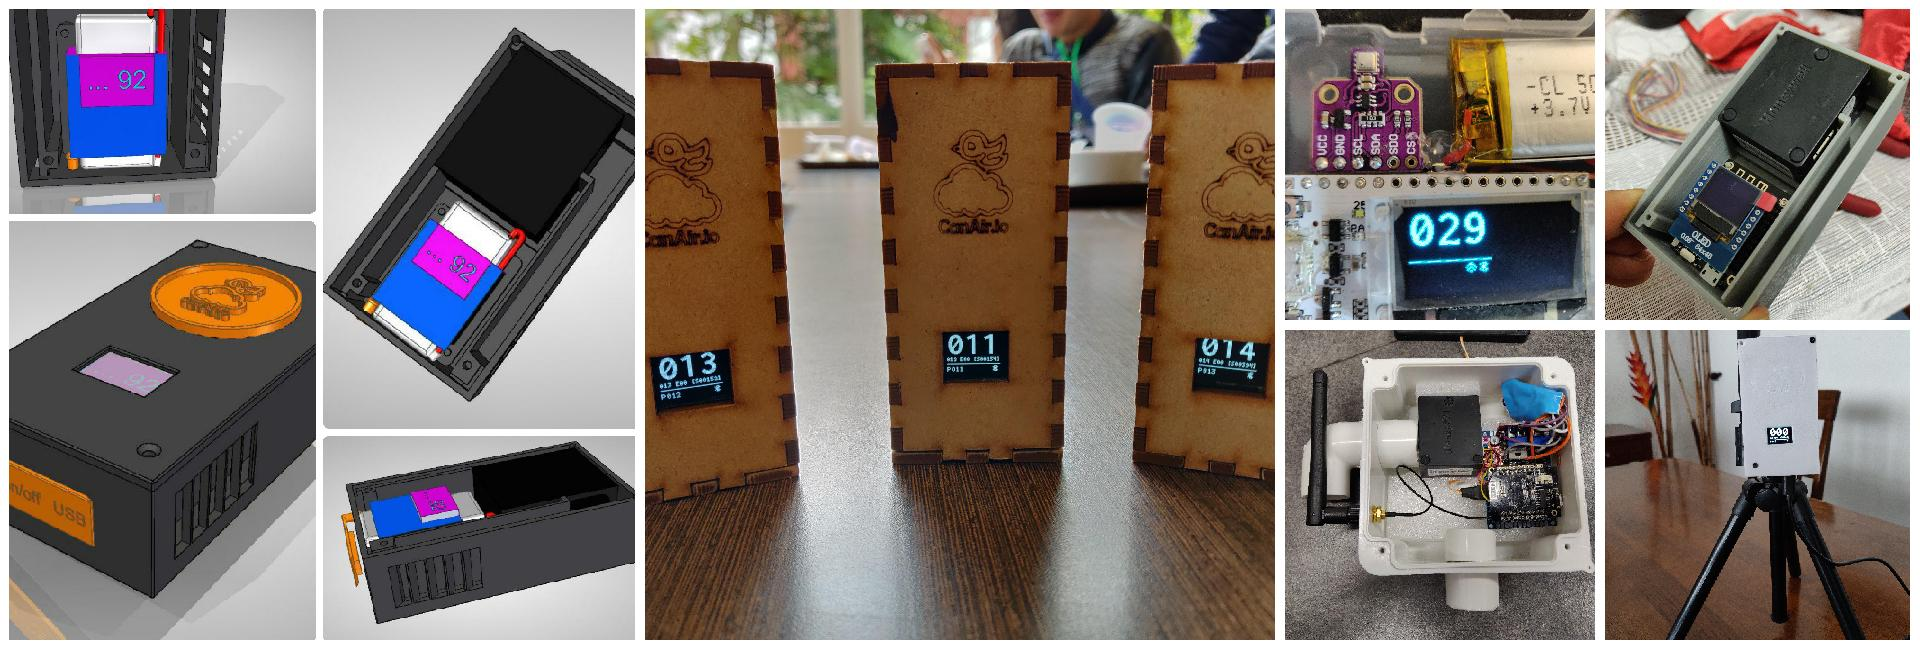
\includegraphics[width=.96\linewidth]{images/collage_horizontal02.jpg} 
  }
  \vspace{0.01cm} %remove this, only added for spacing
}


\headerbox{Citizen work and results}{name=topicoverview,column=0,span=3,below=subtopic2}{
{
    \vspace{0.15cm} %remove this, only added for spacing
    
    {
        \hspace{-.2cm}
        \centering
    	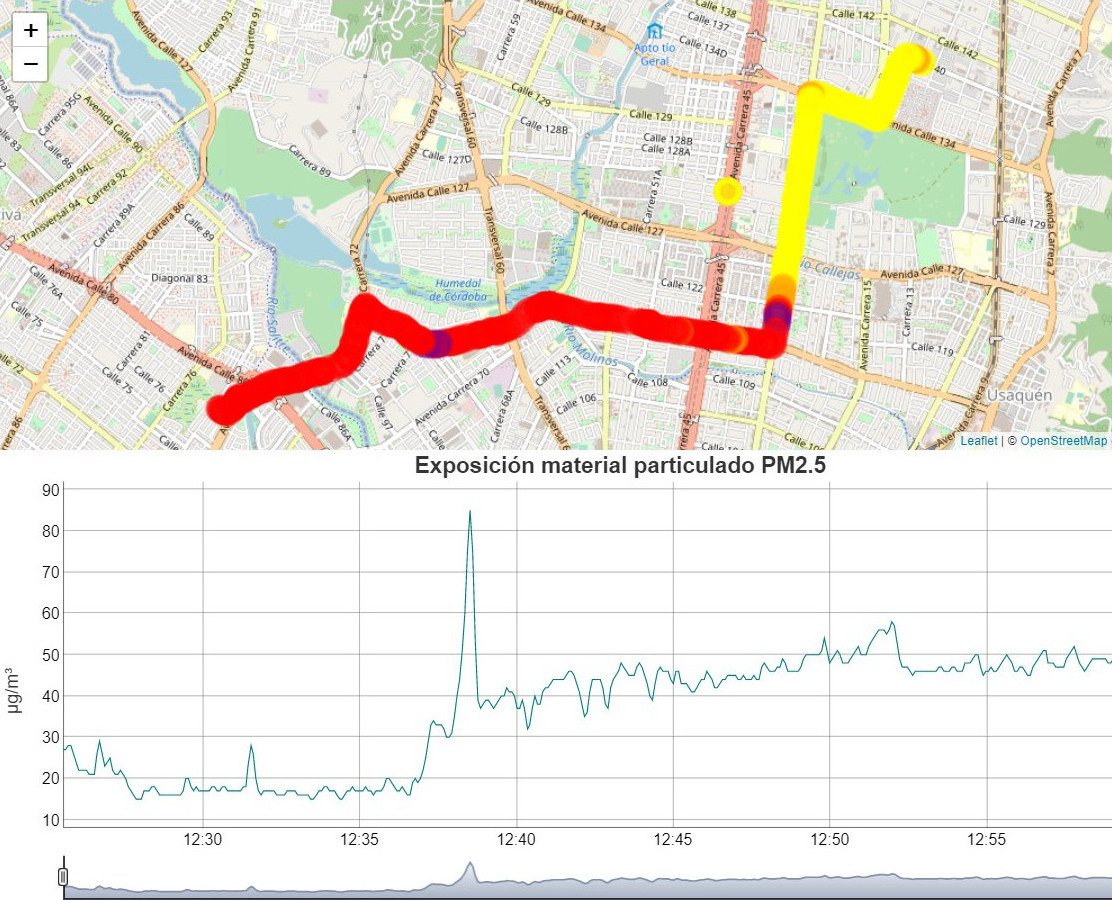
\includegraphics[scale=.82]{images/mobile_capture02.jpg}
    }
    {
        \hspace{-0.3cm}
        \centering
    	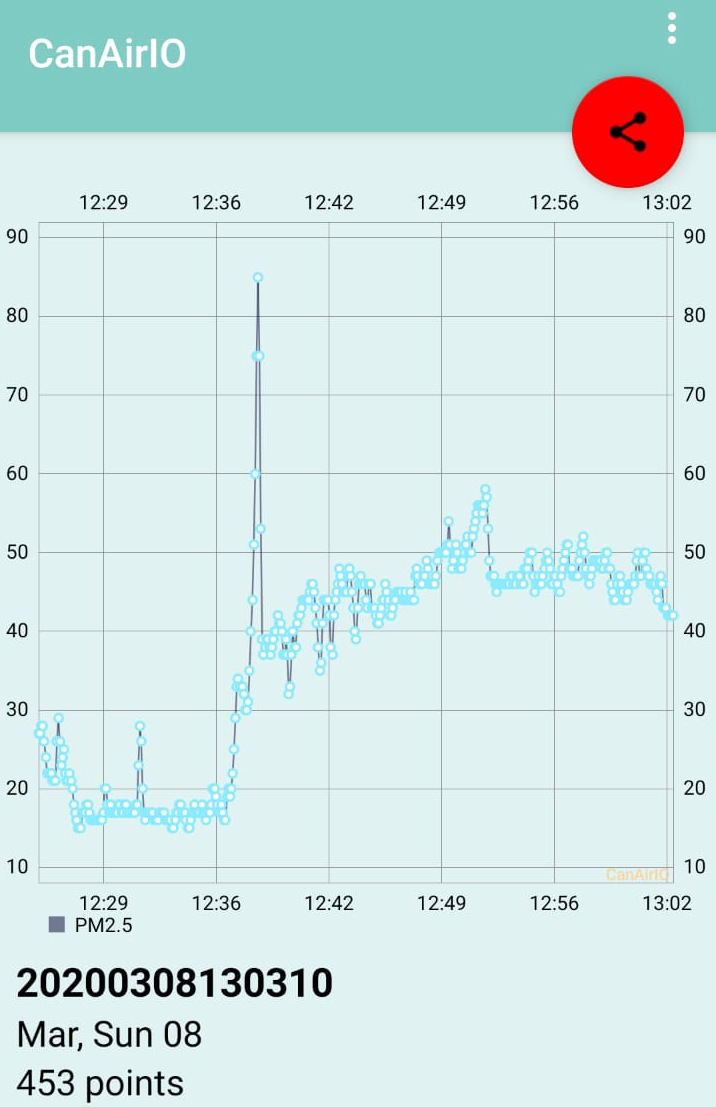
\includegraphics[scale=.16]{images/mobile_capture02_android.jpg}
    }
    {
        \hspace{-0.3cm}
        \centering
    	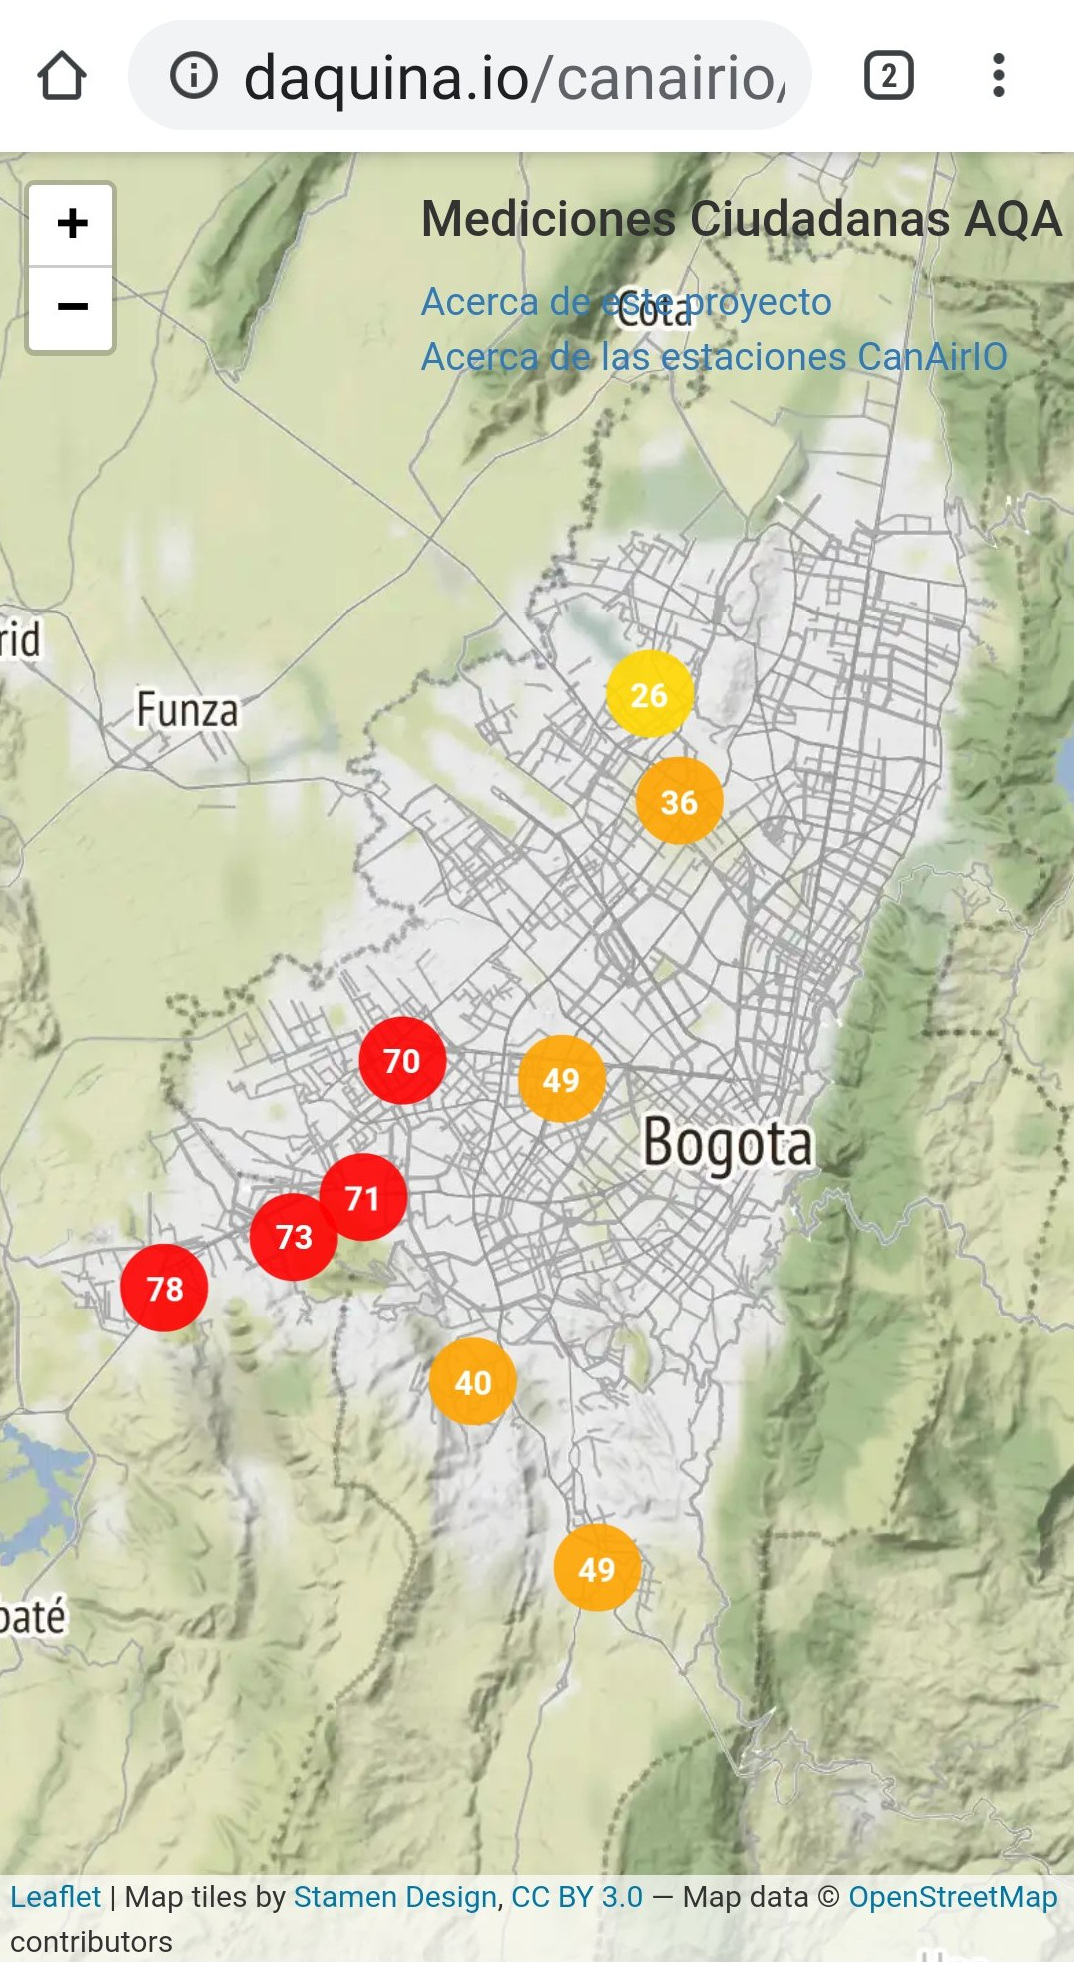
\includegraphics[scale=.38]{images/map_static_stations00.jpg}
    }
    {
        \hspace{-0.3cm}
        \centering
    	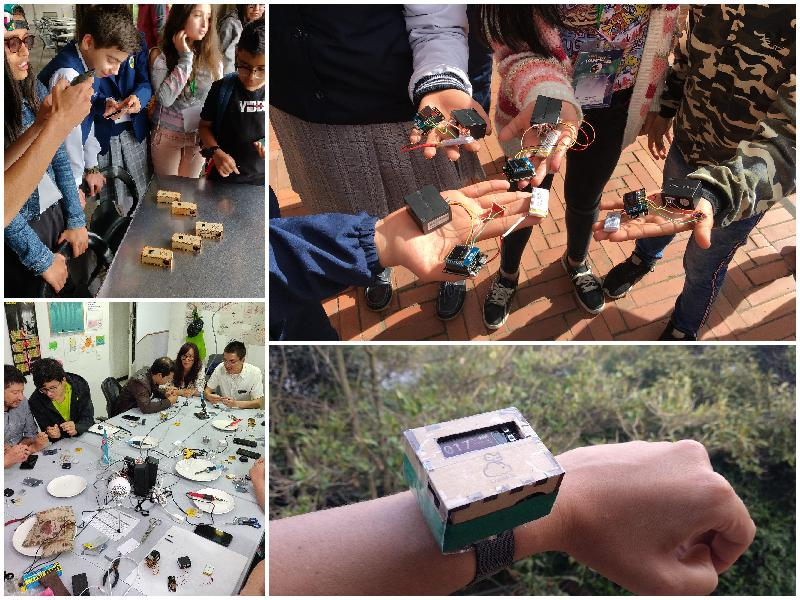
\includegraphics[scale=.295]{images/collage_square00.jpg}
    }

    \vspace{0.15cm} %remove this, only added for spacing

}

}

\headerbox{Thanks to:}{name=thanks,column=0,below=topicoverview,span=1,above=bottom}{

  {
    \subsubsection*{Sponsors:}
    Cos4Cloud: www.cos4cloud-eosc.eu
    \vspace{0.05em}\\
    Trébola: www.trebola.org
    {
      \vspace{-0.2cm}
      \subsubsection*{Communities:}
      Hackbo: hackbo.co
      \vspace{0.05em}\\
      Unloquer: wiki.unloquer.org
      \vspace{0.05em}\\
      Grafoscopio: mutabit.com/grafoscopio
    }
  }

}


\headerbox{Sponsors}{name=sponsors,column=1,below=topicoverview,span=2,above=bottom}{

  {
    {
      \hspace{0.2cm}
      \centering
      
\includegraphics[scale=.65]{images/trebola-logo-01.jpg}
    }
    {
      \hspace{-0.5cm}
      \centering
      
\includegraphics[scale=.13]{images/cos4Cloud_logo-02.png}
    }
    {
      \hspace{-0.5cm}
      \centering
      
\includegraphics[scale=.130]{images/https_canairio.png}
    }
  }

}
\end{poster}

\end{document}
